% !TEX TS-program = pdflatex
% !TEX encoding = UTF-8 Unicode

% This is a simple template for a LaTeX document using the "article" class.
% See "book", "report", "letter" for other types of document.

\documentclass[11pt]{article} % use larger type; default would be 10pt

\usepackage[utf8]{inputenc} % set input encoding (not needed with XeLaTeX)

%%% Examples of Article customizations
% These packages are optional, depending whether you want the features they provide.
% See the LaTeX Companion or other references for full information.

%%% PAGE DIMENSIONS
\usepackage{geometry} % to change the page dimensions
\geometry{a4paper} % or letterpaper (US) or a5paper or....
 \geometry{margin=1in} % for example, change the margins to 2 inches all round
% \geometry{landscape} % set up the page for landscape
%   read geometry.pdf for detailed page layout information

\usepackage{graphicx} % support the \includegraphics command and options

% \usepackage[parfill]{parskip} % Activate to begin paragraphs with an empty line rather than an indent

%%% PACKAGES
\usepackage{booktabs} % for much better looking tables
\usepackage{array} % for better arrays (eg matrices) in maths
\usepackage{paralist} % very flexible & customisable lists (eg. enumerate/itemize, etc.)
\usepackage{verbatim} % adds environment for commenting out blocks of text & for better verbatim
%\usepackage{subfig} % make it possible to include more than one captioned figure/table in a single float
\usepackage{enumitem}
\usepackage{multicol}
\usepackage{tikz}
\usepackage{subcaption}
\usepackage{multirow}
\usepackage[brazilian]{babel}
% These packages are all incorporated in the memoir class to one degree or another...

%%% HEADERS & FOOTERS
\usepackage{fancyhdr} % This should be set AFTER setting up the page geometry
\pagestyle{fancy} % options: empty , plain , fancy
\renewcommand{\headrulewidth}{0pt} % customise the layout...
\lhead{}\chead{Universidade Federal Fluminense\\Departamento de Engenharia Elétrica\\TEE00129 - Laboratório de Eletrônica Básica}\rhead{}
\lfoot{}\cfoot{\thepage}\rfoot{}

%%% SECTION TITLE APPEARANCE
\usepackage{sectsty}
\allsectionsfont{\sffamily\mdseries\upshape} % (See the fntguide.pdf for font help)
% (This matches ConTeXt defaults)

%%% ToC (table of contents) APPEARANCE
\usepackage[nottoc,notlof,notlot]{tocbibind} % Put the bibliography in the ToC
\usepackage[titles,subfigure]{tocloft} % Alter the style of the Table of Contents
\renewcommand{\cftsecfont}{\rmfamily\mdseries\upshape}
\renewcommand{\cftsecpagefont}{\rmfamily\mdseries\upshape} % No bold!

%%% END Article customizations

%%% The "real" document content comes below...

\title{Aula 1: Osciloscópio}
\author{Prof. Derick Furquim Pereira}
\date{} % Activate to display a given date or no date (if empty),
         % otherwise the current date is printed 

\begin{document}
\maketitle
\thispagestyle{fancy}

\begin{enumerate}

\item (4,0 pontos) Calcule o valor médio e o valor eficaz dos sinais abaixo.

\begin{figure}[!h]
    \centering
    \begin{subfigure}[b]{0.45\textwidth}
        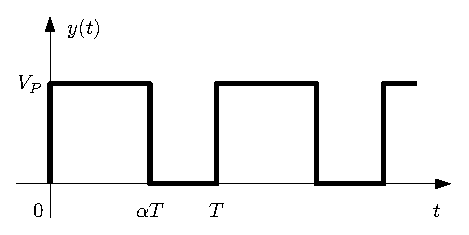
\includegraphics[width=\textwidth]{square.eps}
        \caption{}
    \end{subfigure}
    ~
    \begin{subfigure}[b]{0.45\textwidth}
        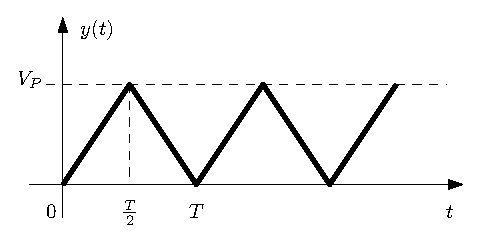
\includegraphics[width=\textwidth]{triangle.eps}
        \caption{}
    \end{subfigure}
\end{figure}

\begin{multicols}{2}
\begin{enumerate}[start=3]
\centering
\item $y(t)=V_P\sin{\omega t}$
\item $y(t)=V_P\sin^2{\omega t}$
\end{enumerate}
\end{multicols}

\item (6,0 pontos) Com o auxílio de um osciloscópio, meça a tensão dos sinais abaixo, esboce a forma de onda observada e meça os valores de pico a pico, eficaz, médio, o período e a frequência.

\begin{enumerate}
\begin{multicols}{2}
\item Sinal de teste interno do osciloscópio
\item Tensão do secundário do transformador da bancada
\end{multicols}
\end{enumerate}

\begin{figure}[!h]
\begin{subfigure}[b]{.45\textwidth}
\centering
\begin{tikzpicture}
\draw[step=.375cm,gray,very thin] (0,0) grid (6,3);
\end{tikzpicture}
\end{subfigure}
~
\begin{subfigure}[b]{.45\textwidth}
\centering
\begin{tikzpicture}
\draw[step=.375cm,gray,very thin] (0,0) grid (6,3);
\end{tikzpicture}
\end{subfigure}
\end{figure}

\begin{table}[!h]
\centering
\caption{Sinal de teste interno do osciloscópio.}
\begin{tabular}{|c|c|c|c|c|}
\hline
Valor & Acoplamento CC & Acoplamento CA & Período & Frequência\\\hline
Pico-pico & & & & \\\cline{1-3}
Eficaz & & & & \\\cline{1-3}
Médio & & & & \\\hline
\end{tabular}
\end{table}

\begin{table}[!h]
\centering
\caption{Tensão do secundário do transformador da bancada.}
\begin{tabular}{|c|c|c|c|c|}
\hline
Valor & Acoplamento CC & Acoplamento CA & Período & Frequência\\\hline
Pico-pico & & & & \\\cline{1-3}
Eficaz & & & & \\\cline{1-3}
Médio & & & & \\\hline
\end{tabular}
\end{table}

\end{enumerate}

\end{document}
